% Use xelatex to generate a pdf file of this presentation
%
% OPENING SLIDES ONLY — title + motivation, built with the Funnel Approach:
% wide industry problem -> Postgres-specific mechanism -> one hidden, concrete
% query. The rest of the deck (The Problem / pg_track_optimizer / results)
% continues after the final divider frame below.

\documentclass{beamer}
\usepackage{roboto}
\usepackage[english]{babel}
\usetheme{Copenhagen}

% Simple way to put a code listing to the slide
\usepackage{listings}

\usepackage{tikz}
\usetikzlibrary{positioning,shapes.geometric}
\usepackage{pgfplots}
\pgfplotsset{compat=1.18}
\usepackage{graphicx}
\usepackage{qrcode}
\usepackage{booktabs}

% --- "The Letter" cold-open slide -------------------------------
% Single static page: the wall of text with one line in red.
\usepackage[most]{tcolorbox}
\definecolor{crash}{HTML}{B21F1F}     % swap for pgorange to stay monochrome
\definecolor{paper}{HTML}{FCFCFA}
\definecolor{mailrule}{HTML}{D8D6D0}
% one log line: \lgl{ink 0-100}{text}
\newcommand{\lgl}[2]{\textcolor{black!#1}{#2}}
% mail header row
\newcommand{\hdr}[2]{%
  \makebox[1.25cm][l]{\textcolor{black!40}{\tiny\textsf{#1}}}%
  \textcolor{black!75}{\tiny\textsf{#2}}\par}
% ----------------------------------------------------------------

% Emblem shown in the corner of every slide, and larger on the title page
\logo{\includegraphics[scale=0.08]{pics/madrid_coat_of_arms}}

% Blocks settings
\setbeamerfont{block title}{size=\tiny}
\setbeamertemplate{navigation symbols}{}

%Information to be included in the title page:
\title{When the Planner's Misestimation Inflates Your Cloud Bill}
\subtitle{Finding the Costly Queries \texttt{pg\_stat\_statements} Can't See}
\author{Andrei Lepikhov}
\institute{pgEdge}
\date{PGDay Israel, 25.10.2026}

% Add page numbers in the footnote
\expandafter\def\expandafter\insertshorttitle\expandafter{%
  \insertshorttitle\hfill%
  \insertframenumber\,/\,\inserttotalframenumber}

\definecolor{lightlightgray}{gray}{0.9}
\definecolor{pgblue}{HTML}{336791}
\definecolor{pgorange}{HTML}{E8781A}

% Default listing format
\lstset{language=sql, frame=none, tabsize=2, identifierstyle=\color{black},
  showspaces=false, showtabs=false, showstringspaces=false,
  columns=fullflexible, % Restore default spaces between letters
  basicstyle=\rmfamily\scriptsize,
  stringstyle=\color{purple},
  keywordstyle=\bfseries\color{green!40!black},
  numberstyle=\tiny\color{gray},
  morekeywords={PUBLICATION,SUBSCRIPTION,CONNECTION,WITH,COPY,FORMAT}}

% -----------------------------

\begin{document}

% %%%%%%%%%%%%%%%%%%%%%%%%%%%%%%%%%%%%%%%%%%%%%%%%%%%%%%%%%%%%%%%%%%%%%%%%
% Title
% %%%%%%%%%%%%%%%%%%%%%%%%%%%%%%%%%%%%%%%%%%%%%%%%%%%%%%%%%%%%%%%%%%%%%%%%

\begin{frame}
\titlepage
\end{frame}

% %%%%%%%%%%%%%%%%%%%%%%%%%%%%%%%%%%%%%%%%%%%%%%%%%%%%%%%%%%%%%%%%%%%%%%%%
% Cold open: the letter that started the investigation
% %%%%%%%%%%%%%%%%%%%%%%%%%%%%%%%%%%%%%%%%%%%%%%%%%%%%%%%%%%%%%%%%%%%%%%%%

\begin{frame}[fragile]\frametitle{31 December 2023}

\vspace{-0.6em}
\hfill{\tiny\textsf{\textcolor{black!45}{pgsql-bugs@lists.postgresql.org}}}

\vspace{-0.9em}

\begin{tcolorbox}[
  enhanced, sharp corners=downhill, arc=1pt,
  colback=paper, colframe=mailrule, boxrule=0.4pt,
  left=6pt, right=6pt, top=5pt, bottom=2pt,
  drop shadow={black!12}]

\hdr{From}{Michael B. Williams
           \textcolor{black!35}{$\langle$michael.williams@glexia.com$\rangle$}}
\hdr{Subject}{\textbf{Segmentation fault caused by Postgrest -
              reateplan.c:6178 - prepare\_sort\_from\_pathkeys}}

\vspace{-1pt}\textcolor{mailrule}{\hrule height 0.4pt}\vspace{6pt}

{\ttfamily\fontsize{6.8}{9.0}\selectfont
 \setlength{\parskip}{0pt}\setlength{\topsep}{0pt}\setlength{\partopsep}{0pt}
\begin{semiverbatim}
\lgl{62}{2023-12-31 03:23:12.048 PST [17763] LOG: server process (PID 19014) was}
\lgl{62}{terminated by \textcolor{crash}{signal 11: Segmentation fault}}
\lgl{62}{2023-12-31 03:23:12.048 PST [17763] DETAIL: Failed process was running:}
\lgl{50}{      with recursive}
\lgl{48}{      pks_fks as (}
\lgl{34}{        -- pk + fk referencing col}
\lgl{44}{        select}
\lgl{40}{          contype::text as contype,}
\lgl{36}{          conname,}
\lgl{31}{          array_length(conkey, 1) as ncol,}
\lgl{26}{          conrelid as resorigtbl,}
\lgl{21}{          col as resorigcol,}
\lgl{16}{          ord}
\lgl{12}{        from pg_constraint}
\lgl{8}{        left join lateral unnest(conkey) with ordinality as _(col, ord)}
\lgl{4}{        where contype IN ('p', 'f')}
\end{semiverbatim}
}
\end{tcolorbox}

\vspace{-0.7em}\hspace{0.8cm}
{\tiny\textsf{\textcolor{black!30}{$\vdots$\quad and then the whole gdb session: \#0 \ldots\ \#21}}}

\end{frame}

% %%%%%%%%%%%%%%%%%%%%%%%%%%%%%%%%%%%%%%%%%%%%%%%%%%%%%%%%%%%%%%%%%%%%%%%%
% Why This Matters
% %%%%%%%%%%%%%%%%%%%%%%%%%%%%%%%%%%%%%%%%%%%%%%%%%%%%%%%%%%%%%%%%%%%%%%%%

\begin{frame}
\vspace*{\fill}\begin{center}
\huge{Why This Matters}
\end{center}\vspace*{\fill}
\end{frame}

\begin{frame}\frametitle{Motivation}
\small
\textbf{1. Cloud database spend is already under scrutiny.}\\
Industry estimates put 20--60\% of cloud data spend as avoidable ---
and Postgres is not exempt: one team cut its AWS RDS bill by 59\%
after tuning.
{\tiny\textit{(Revefi, Xomnia; Brocoders --- AWS RDS PostgreSQL case)}}

\medskip
\textbf{2. The standard practice only sees what's already loud.}\\
Sort \texttt{pg\_stat\_statements} by total time, fix the worst
offender, deploy. It works --- but a query that takes 20\,ms and runs
ten million times a day never makes that list, even though it should
run in 2\,ms.

\medskip
\textbf{3. The root cause hides in a single wrong number.}\\
A bad row estimate makes the planner pick a plan that looks
``good enough'' --- a nested loop instead of a hash join, a scan
wider than it needs to be. At low volume nobody notices. At scale it
quietly burns CPU and I/O every day, never showing up as a slow
query.

\medskip
{\textit{On one production system, a query executing in 0.39\,ms was
called 1\,824 times --- with a cardinality estimate off by roughly
5\,000$\times$. Nothing here looks slow. Everything here is about to
become expensive.}}
\end{frame}

% %%%%%%%%%%%%%%%%%%%%%%%%%%%%%%%%%%%%%%%%%%%%%%%%%%%%%%%%%%%%%%%%%%%%%%%%
% The Funnel: from industry noise to one hidden query
% %%%%%%%%%%%%%%%%%%%%%%%%%%%%%%%%%%%%%%%%%%%%%%%%%%%%%%%%%%%%%%%%%%%%%%%%

\begin{frame}\frametitle{Narrowing Down: Where the Real Cost Hides}
\begin{center}
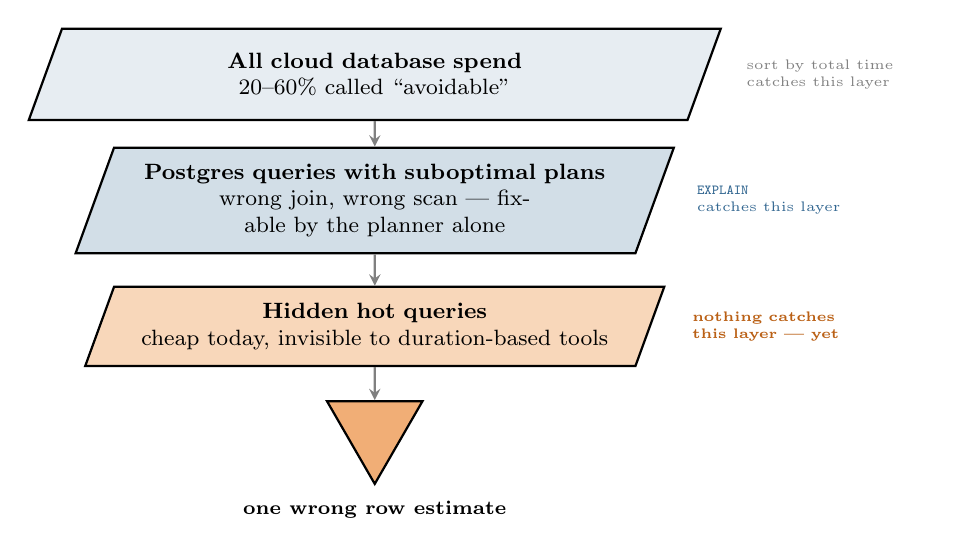
\begin{tikzpicture}[
  band/.style={trapezium, draw, thick, trapezium left angle=70,
               trapezium right angle=110, align=center,
               font=\footnotesize, inner sep=6pt, text width=6.2cm},
  lbl/.style={font=\tiny, text=gray, align=left, text width=2.4cm},
  arr/.style={->, thick, >=stealth, gray},
]

\node[band, minimum width=8.8cm, fill=pgblue!12] (b1) at (0,0)
  {\textbf{All cloud database spend}\\{\footnotesize 20--60\% called ``avoidable''}};

\node[band, minimum width=7cm, fill=pgblue!22] (b2) at (0,-1.6)
  {\textbf{Postgres queries with suboptimal plans}\\{\footnotesize wrong join, wrong scan --- fixable by the planner alone}};

\node[band, minimum width=4.6cm, fill=pgorange!30] (b3) at (0,-3.2)
  {\textbf{Hidden hot queries}\\{\footnotesize cheap today, invisible to duration-based tools}};

\node[regular polygon, regular polygon sides=3, shape border rotate=180,
      draw, thick, fill=pgorange!60, minimum width=1.4cm] (tip) at (0,-4.5) {};
\node[font=\scriptsize\bfseries, below=2pt of tip] {one wrong row estimate};

\draw[arr] (b1) -- (b2);
\draw[arr] (b2) -- (b3);
\draw[arr] (b3) -- (tip);

\node[lbl, right=0.4cm of b1] {sort by total time\\catches this layer};
\node[lbl, right=0.4cm of b2, text=pgblue] {\texttt{EXPLAIN}\\catches this layer};
\node[lbl, right=0.4cm of b3, text=pgorange!80!black] {\textbf{nothing catches\\this layer --- yet}};

\end{tikzpicture}
\end{center}
\end{frame}

% %%%%%%%%%%%%%%%%%%%%%%%%%%%%%%%%%%%%%%%%%%%%%%%%%%%%%%%%%%%%%%%%%%%%%%%%
% The Problem  (section continues elsewhere in the full deck)
% %%%%%%%%%%%%%%%%%%%%%%%%%%%%%%%%%%%%%%%%%%%%%%%%%%%%%%%%%%%%%%%%%%%%%%%%

\begin{frame}
\vspace*{\fill}\begin{center}
\huge{The Problem}
\end{center}\vspace*{\fill}
\end{frame}

\end{document}
